\begin{center}
\begin{tikzpicture}
	\node[anchor=south west,inner sep=0] (image)  at (0,0) {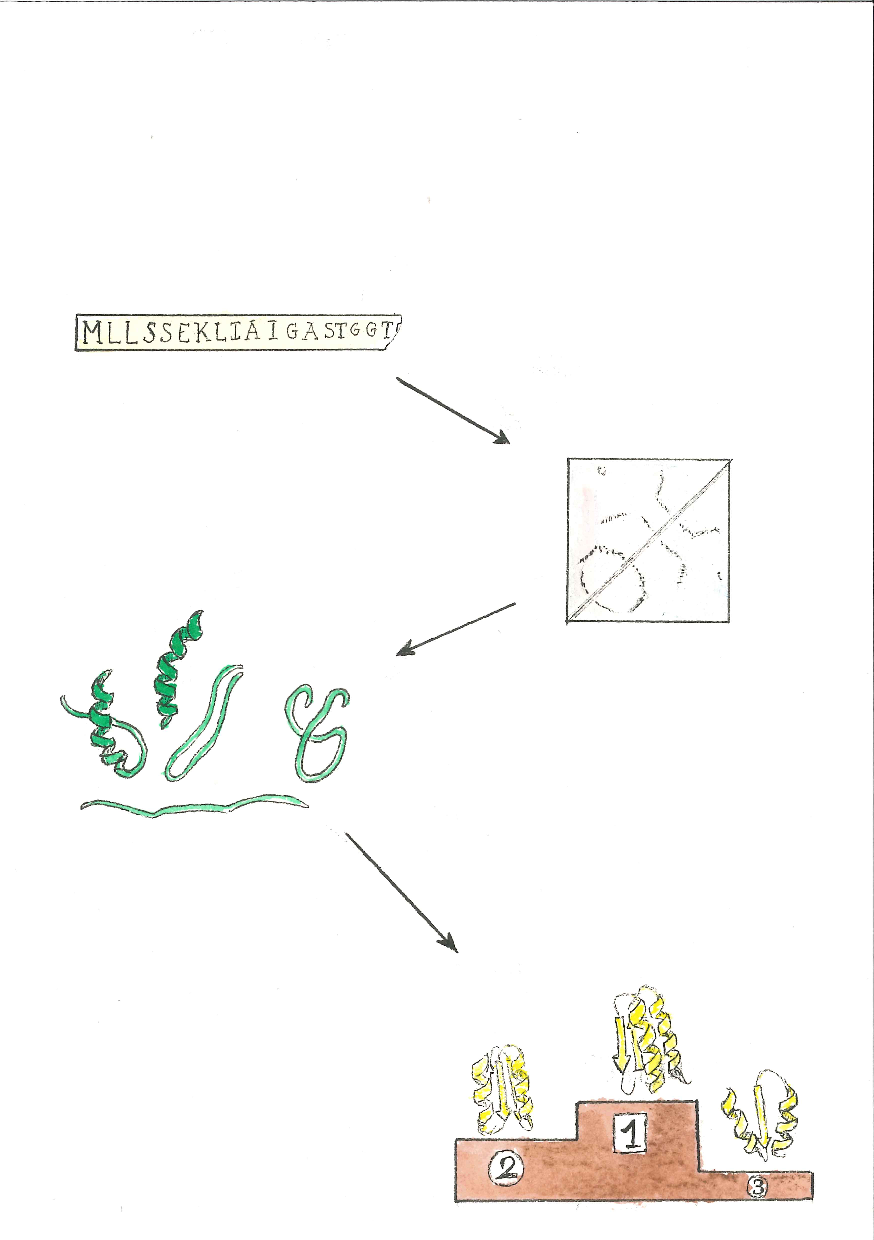
\includegraphics[trim={2mm, 2mm, 2mm, 2mm}, width=0.985\pagewidth]{scans/panel-8.pdf}};
    \begin{scope}[x={(current page.south east)},y={(current page.north west)}]
		\if\helplines1
			\draw[help lines,xstep=.1,ystep=.1] (0,0) grid (\N, \N);
		\else
			\path[help lines,xstep=.1,ystep=.1] (0,0) grid (\N, \N);
		\fi
		\node(title) at (0.5, 0.9) {\Huge {\color{Maroon}II} - PconsFold2};
		
		\node[align=center](a) at (0.5, 0.85) {\english{In this paper, we built a pipeline for protein \emph{ab initio} structure prediction.}};
		
		\node[anchor=north](b) at (0.7, 0.76) {\english{From the sequence...}};
		\node[anchor=south](c) at (0.25, 0.6) {\english{...we predict the contacts...}};
		\node[anchor=north](d) at (0.70, 0.44) {\english{...use them to build a pool of models...}};
		\node[anchor=north](e) at (0.25, 0.15) {\english{...and we pick the best ones.}};

		\node[align=center, text width=0.9\pagewidth, align=center, below=2mm of a] {\spanish{En este artículo, desarrollamos un proceso para predecir\\ estructuras de proteínas \emph{ab-initio}}};
		\node[anchor=north, below=3mm of b]  {\spanish{Empezando con la secuencia...}};
		\node[anchor=north, below=3mm of c] {\spanish{...predecimos los contactos...}};
		\node[anchor=north, below=3mm of d] {\spanish{...los usamos para crear un grupo de modelos...}};
		\node[anchor=nort, below=3mm of e]  {\spanish{...y escogemos los mejores.}};

    \end{scope}

\end{tikzpicture}
\end{center}
